\documentclass{beamer}

\usepackage{graphicx}
\usepackage[utf8]{inputenc}
\usepackage[T1]{fontenc}
\usepackage{lmodern}
\usepackage[english]{babel}
\usepackage{amsmath}
\usepackage{amsthm}
\usepackage{mathtools}
\usepackage{amssymb}
\usepackage{listings}
\usepackage{xparse}
\usepackage{stmaryrd}
\usepackage{geometry}
\usepackage{enumerate}
\usepackage{hyperref}
\usepackage{tikz}
\usepackage{pgfplots}
\usepackage{stmaryrd}
\usepackage[style=english]{csquotes}
\usepackage[language=english, backend=biber, style=alphabetic, sorting=nyt]{biblatex}

\hypersetup{
    colorlinks,
    linkcolor={red!50!black},
    citecolor={blue!50!black},
    urlcolor={blue!80!black}
}

\usetikzlibrary{babel, positioning, shapes.geometric, arrows, arrows.meta}
\addbibresource{bibliography.bib}

\title{Classic Paper Reading Group Session 2\\~\\On the role of definitions in and beyond cryptography \cite{role_of_definitions}}
\author{Simon Pohmann}

\newcommand{\Z}{\mathbb{Z}}
\newcommand{\F}{\mathbb{F}}
\newcommand{\C}{\mathbb{C}}
\newcommand{\I}{\mathbb{I}}
\newcommand{\V}{\mathbb{V}}
\newcommand{\End}{\mathrm{End}}
\newcommand{\Quot}{\mathrm{Quot}}
\newcommand{\Half}{\mathcal{H}}
\newcommand{\Lattice}{\mathcal{L}}
\newcommand{\divides}{\ \mid \ }
\newcommand{\notdivides}{\ \nmid \ }
\newcommand{\Cl}{\mathrm{Cl}}
\newcommand{\K}{\mathcal{K}}
\newcommand{\p}{\mathfrak{p}}
\newcommand{\q}{\mathfrak{q}}
\newcommand{\val}{v}
\renewcommand{\l}{\mathfrak{l}}
\renewcommand{\a}{\mathfrak{a}}
\renewcommand{\b}{\mathfrak{b}}
\renewcommand{\O}{\mathcal{O}}

\newcommand\restr[2]{{
    \left.\kern-\nulldelimiterspace
    #1
    \vphantom{\big|}
    \right|_{#2}
}}

\newtheorem{remark}{Remark}

\begin{document}

\begin{frame}
    \maketitle
\end{frame}

\begin{frame}
    \frametitle{Pseudorandom number generators}
    \begin{center}
        When should we consider a sequence of numbers to be ``random''?
    \end{center}
    \pause
    \begin{definition}
        A function $G: \{ 0, 1 \}^n \to \{ 0, 1 \}^N$ with $N > n \geq 1$ is called \emph{pseudorandom generator}.
    \end{definition}
    \pause
    \begin{remark}
        PRG are more like ``randomness expanders''
    \end{remark}
\end{frame}

\begin{frame}
    \frametitle{``How random'' is a PRG?}
    \begin{definition}
        The advantage of an algorithm $A$ when attacking a PRG $G$ is
        \begin{equation*}
            \text{\textbf{Adv}}_G^{\text{PRG}}(A) := \Pr[\text{\textbf{Game}}_G^0(A) = 0] - \Pr[\text{\textbf{Game}}_G^1(A) = 0]
        \end{equation*}
        in
        \\~\\
        \begin{minipage}{0.5\textwidth}
            {\begin{center}
                $\text{\textbf{Game}}_G^0(A)$

                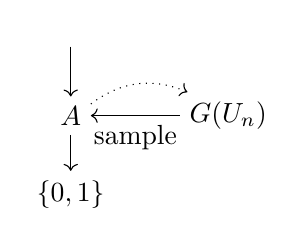
\begin{tikzpicture}
                    \node (begin) at (0, 0) {};
                    \node (A) at (0, -1) {$A$};
                    \node (X) at (2, -1) {$G(U_n)$};
                    \node (end) at (0, -2) {$\{ 0, 1 \}$};
    
                    \draw [->] (begin) -- (A);
                    \draw [->] (A) -- (end);
                    \draw [dotted, ->] (A) to [bend left] (X);
                    \draw [->] (X) -- (A) node [midway, below] {sample};
                \end{tikzpicture}
            \end{center}}
        \end{minipage}%
        \begin{minipage}{0.5\textwidth}
            {\begin{center}
                $\text{\textbf{Game}}_G^1(A)$

                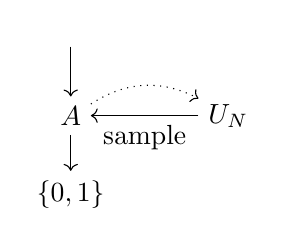
\begin{tikzpicture}
                    \node (begin) at (0, 0) {};
                    \node (A) at (0, -1) {$A$};
                    \node (X) at (2, -1) {$U_N$};
                    \node (end) at (0, -2) {$\{ 0, 1 \}$};
    
                    \draw [->] (begin) -- (A);
                    \draw [->] (A) -- (end);
                    \draw [dotted, ->] (A) to [bend left] (X);
                    \draw [->] (X) -- (A) node [midway, below] {sample};
                \end{tikzpicture}
            \end{center}}
        \end{minipage}
        \\~\\
        where $U_n$ resp. $U_N$ are uniformly random.
    \end{definition}
\end{frame}

\begin{frame}
    \frametitle{Provable security}

    \begin{example}
        If $G: \{ 0, 1 \}^n \to \{ 0, 1 \}^{n + 1}$ is a PRG, then this is also the case for
        \begin{center}
            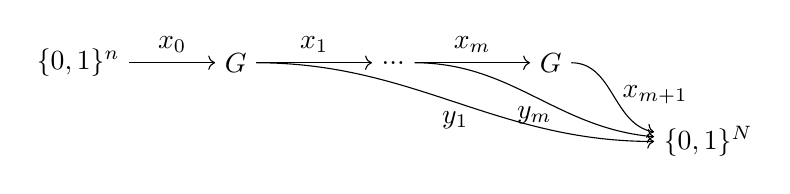
\begin{tikzpicture}
                \node (in) at (0, 0) {$\{ 0, 1 \}^n$};
                \node (expandstart) at (2, 0) {$G$};
                \node (expandmid) at (4, 0) { ... };
                \node (expandend) at (6, 0) {$G$};
                \node (out) at (8, -1) {$\{0, 1\}^N$};

                \draw [->] (in) -- (expandstart) node [midway, above] {$x_0$};
                \draw [->] (expandstart) -- (expandmid) node [midway, above] {$x_1$};
                \draw [->] (expandstart) to [out = 0, in = 180] node [midway, below] {$y_1$} (out);
                
                \draw [->] (expandmid) -- (expandend) node [midway, above] {$x_m$};
                \draw [->] (expandmid) to [out = 0, in = 175] node [midway, below] {$y_m$} (out);

                \draw [->] (expandend) to [out = 0, in = 170] node [midway, right] {$x_{m + 1}$} (out);
            \end{tikzpicture}
        \end{center}
    \end{example}
    \textbf{Proof:} \cite[Thm.~8.19]{katz_lindell}

    \vspace{20pt}

    \begin{itemize}
        \item<2-> Definitions have a huge impact on the field
        \item<3-> Definitions are about ideas
        \item<4-> Good definitions are robust 
    \end{itemize}
\end{frame}

\begin{frame}
    \frametitle{Asymptotic notions}

    \begin{definition}
        A function $f: \Z_+ \to \mathbb{R}_+$ is \emph{negligible}, if $f(n)$ is \emph{eventually} smaller than any $1/\mathrm{poly(n)}$.
    \end{definition}

    \begin{definition}
        An algorithm $A$ is \emph{polynomial-time}, if there is a polynomial $p$ such that the number of operations on an input of length $n$ is at most $p(n)$.
    \end{definition}

    \begin{center}
        \begin{minipage}{0.5\textwidth}
            \begin{tikzpicture}
                \begin{axis}[
                    width = \textwidth, 
                    height = 0.5\textheight, 
                    axis lines = middle,
                    xlabel = $n$,
                    ylabel = $y$
                ]
                    \addplot [red, thick, domain=0:5] {x^4};
                    \addplot [blue, thick, domain=0:5] {exp(x)};
                \end{axis}
            \end{tikzpicture}
        \end{minipage}%
        \uncover<2->{\begin{minipage}{0.5\textwidth}
            \begin{tikzpicture}
                \begin{axis}[
                    width = \textwidth, 
                    height = 0.5\textheight, 
                    axis lines = middle,
                    samples = 1000,
                    xlabel = $n$,
                    ylabel = $y$
                ]
                    \addplot [red, thick, domain=0:50] {x^4};
                    \addplot [blue, thick, domain=0:50] {exp(x)};
                \end{axis}
            \end{tikzpicture}
        \end{minipage}}%
    \end{center}
\end{frame}

\begin{frame}
    \frametitle{Asymptotic and concrete security}
    {
        \def\arraystretch{1.5}
        \begin{tabular}{c | c}
            Concrete & Asymptotic \\
            \hline
            application oriented & originated in complexity theory \\
            \uncover<2->{no definition of ``secure''} & \uncover<2->{secure $:=$ advantage is negligible} \\
            \uncover<3->{constant in/output size} & \uncover<3->{sizes depend on ``security parameter''} \\
            \uncover<4->{attackers must be ``feasible''} & \uncover<4->{attackers must be polynomial-time}
        \end{tabular}
    }

    \vspace{20pt}

    \begin{itemize}
        \item<5-> Definitions can change the way a theory develops
        \item<6-> Definitions come from a scientific culture
    \end{itemize}
\end{frame}

\begin{frame}
    \frametitle{Blockciphers}

    \begin{definition}
        A \emph{blockcipher} is a function $E: \mathcal{K} \times \{0, 1\}^n \to \{0, 1\}^n$ such that $E(k, \cdot)$ is a permutation for all $k \in \mathcal{K}$.
    \end{definition}

    \begin{center}
        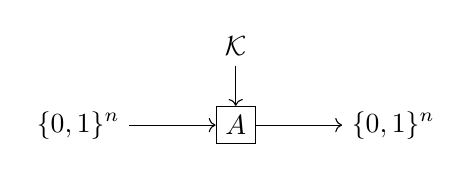
\begin{tikzpicture}
            \node (begin) at (0, -1) {$\{0, 1\}^n$};
            \node (key) at (2, 0) {$\mathcal{K}$};
            \node [shape = rectangle, draw = black] (X) at (2, -1) {$A$};
            \node (end) at (4, -1) {$\{ 0, 1 \}^n$};

            \draw [->] (begin) -- (X);
            \draw [->] (key) -- (X);
            \draw [->] (X) -- (end);
        \end{tikzpicture}
    \end{center}

    \uncover<2->{\begin{remark}
        We did not specify the decryption function.
    \end{remark}}
\end{frame}

\begin{frame}
    \frametitle{Advantage for blockciphers}

    \begin{definition}
        The advantage of an algorithm $A$ during a \emph{chosen-ciphertext attack} to blockcipher $E$ is
        \begin{equation*}
            \text{\textbf{Adv}}_E^{\text{CPA}}(A) := \Pr[\text{\textbf{Game}}_E^0(A, k) = 0] - \Pr[\text{\textbf{Game}}_E^1(A, \pi) = 0]
        \end{equation*}
        for a uniformly random $k \in \mathcal{K}$ and $\pi \in \mathrm{Sym}(\{0, 1\}^n)$ in the games
        \\~\\
        \begin{minipage}{0.5\textwidth}
            \begin{center}
                $\text{\textbf{Game}}_E^0(A, k)$
                \\~\\
                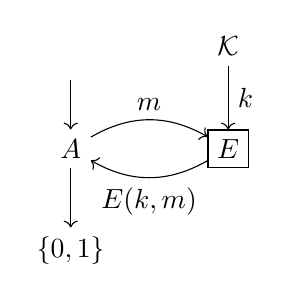
\begin{tikzpicture}
                    \node (begin) at (0, 0) {};
                    \node (key) at (2, 0.3) {$\mathcal{K}$};
                    \node (A) at (0, -1) {$A$};
                    \node [shape = rectangle, draw = black] (X) at (2, -1) {$E$};
                    \node (end) at (0, -2.3) {$\{ 0, 1 \}$};
    
                    \draw [->] (begin) -- (A);
                    \draw [->] (A) -- (end);
                    \draw [->] (key) -- (X) node [midway, right] {$k$};
                    \draw [->] (A) to [bend left] node [above, midway] {$m$} (X);
                    \draw [->] (X) to [bend left] node [below, midway] {$E(k, m)$} (A);
                \end{tikzpicture}
            \end{center}
        \end{minipage}%
        \begin{minipage}{0.5\textwidth}
            \begin{center}
                $\text{\textbf{Game}}_E^1(A, \pi)$
                \\~\\
                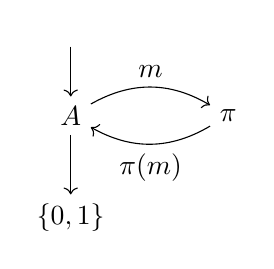
\begin{tikzpicture}
                    \node (begin) at (0, 0) {};
                    \node (A) at (0, -1) {$A$};
                    \node (X) at (2, -1) {$\pi$};
                    \node (end) at (0, -2.3) {$\{ 0, 1 \}$};
    
                    \draw [->] (begin) -- (A);
                    \draw [->] (A) -- (end);
                    \draw [->] (A) to [bend left] node [above, midway] {$m$} (X);
                    \draw [->] (X) to [bend left] node [below, midway] {$\pi(m)$} (A);
                \end{tikzpicture}
            \end{center}
        \end{minipage}
    \end{definition}
\end{frame}

\begin{frame}
    \frametitle{Advantage for blockciphers}

    \begin{minipage}{0.5\textwidth}
        \begin{center}
            $\text{\textbf{Game}}_E^0(A, k)$
            \\~\\
            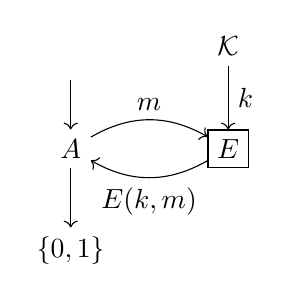
\begin{tikzpicture}
                \node (begin) at (0, 0) {};
                \node (key) at (2, 0.3) {$\mathcal{K}$};
                \node (A) at (0, -1) {$A$};
                \node [shape = rectangle, draw = black] (X) at (2, -1) {$E$};
                \node (end) at (0, -2.3) {$\{ 0, 1 \}$};

                \draw [->] (begin) -- (A);
                \draw [->] (A) -- (end);
                \draw [->] (key) -- (X) node [midway, right] {$k$};
                \draw [->] (A) to [bend left] node [above, midway] {$m$} (X);
                \draw [->] (X) to [bend left] node [below, midway] {$E(k, m)$} (A);
            \end{tikzpicture}
        \end{center}
    \end{minipage}%
    \begin{minipage}{0.5\textwidth}
        \begin{center}
            $\text{\textbf{Game}}_E^1(A, \pi)$
            \\~\\
            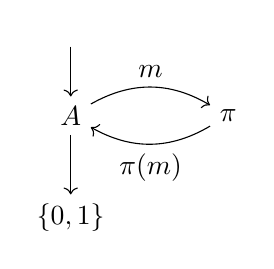
\begin{tikzpicture}
                \node (begin) at (0, 0) {};
                \node (A) at (0, -1) {$A$};
                \node (X) at (2, -1) {$\pi$};
                \node (end) at (0, -2.3) {$\{ 0, 1 \}$};

                \draw [->] (begin) -- (A);
                \draw [->] (A) -- (end);
                \draw [->] (A) to [bend left] node [above, midway] {$m$} (X);
                \draw [->] (X) to [bend left] node [below, midway] {$\pi(m)$} (A);
            \end{tikzpicture}
        \end{center}
    \end{minipage}

    \vspace{20pt}

    \begin{itemize}
        \item<2-> For low-level primitives, simple \& pessimistic definitions are better
    \end{itemize}
\end{frame}

\begin{frame}
    \frametitle{Authenticated Encryption}

    \begin{definition}
        An AE scheme are two deterministic functions
        \begin{align*}
            &E: \mathcal{K} \times \mathcal{N} \times \{ 0, 1 \}^* \to \{ 0, 1 \}^* \quad \text{(encryption)}\\
            &D: \mathcal{K} \times \mathcal{N} \times \{ 0, 1 \}^* \cup \{ \perp \} \quad \text{(decryption)}
        \end{align*}
        such that $D(k, n, E(k, n, m)) = m$ for all $k, n, m$.
        Further, we require that $|E(k, n, m)| = |m| = \tau$.
    \end{definition}
    \begin{center}
        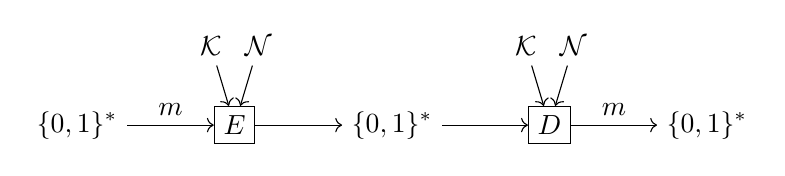
\begin{tikzpicture}
            \node (begin) at (0, -1) {$\{ 0, 1 \}^*$};
            \node (key) at (1.7, 0) {$\mathcal{K}$};
            \node (nonce) at (2.3, 0) {$\mathcal{N}$};
            \node [shape = rectangle, draw = black] (X) at (2, -1) {$E$};
            \node (transmission) at (4, -1) {$\{ 0, 1 \}^*$};
            \node [shape = rectangle, draw = black] (X2) at (6, -1) {$D$};
            \node (key2) at (5.7, 0) {$\mathcal{K}$};
            \node (nonce2) at (6.3, 0) {$\mathcal{N}$};
            \node (end) at (8, -1) {$\{ 0, 1 \}^*$};
            
            \draw [->] (begin) -- (X) node [midway, above] {$m$};
            \draw [->] (key) -- (X);
            \draw [->] (nonce) -- (X);
            \draw [->] (X) -- (transmission);
            \draw [->] (transmission) -- (X2);
            \draw [->] (key2) -- (X2);
            \draw [->] (nonce2) -- (X2);
            \draw [->] (X2) -- (end) node [midway, above] {$m$};
        \end{tikzpicture}
    \end{center}
\end{frame}

\begin{frame}
    \frametitle{Two contests}
    \begin{definition}[privacy advantage]
        The advantage of an algorithm $A$ for a privacy attack on an AE scheme $(E, D)$ is
        \begin{equation*}
            \text{\textbf{Adv}}_E^{\text{AE-P}}(A) := \Pr[\text{\textbf{Game}}_E^0(A, k) = 0] - \Pr[\text{\textbf{Game}}_E^1(A) = 0]
        \end{equation*}
        for a uniformly random $k \in \mathcal{K}$ in the games
        \\~\\
        \begin{minipage}{0.5\textwidth}
            \begin{center}
                $\text{\textbf{Game}}_E^0(A, k)$
                \\~\\
                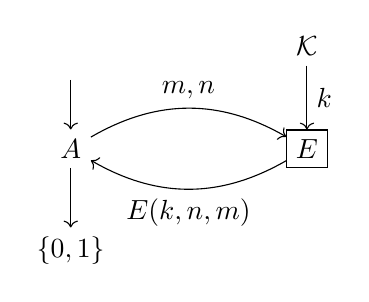
\begin{tikzpicture}
                    \node (begin) at (0, 0) {};
                    \node (key) at (3, 0.3) {$\mathcal{K}$};
                    \node (A) at (0, -1) {$A$};
                    \node [shape = rectangle, draw = black] (X) at (3, -1) {$E$};
                    \node (end) at (0, -2.3) {$\{ 0, 1 \}$};
    
                    \draw [->] (begin) -- (A);
                    \draw [->] (A) -- (end);
                    \draw [->] (key) -- (X) node [midway, right] {$k$};
                    \draw [->] (A) to [bend left] node [above, midway] {$m, n$} (X);
                    \draw [->] (X) to [bend left] node [below, midway] {$E(k, n, m)$} (A);
                \end{tikzpicture}
            \end{center}
        \end{minipage}%
        \begin{minipage}{0.5\textwidth}
            \begin{center}
                $\text{\textbf{Game}}_E^1(A, \pi)$
                \\~\\
                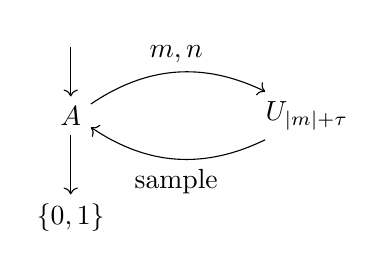
\begin{tikzpicture}
                    \node (begin) at (0, 0) {};
                    \node (A) at (0, -1) {$A$};
                    \node (X) at (3, -1) {$U_{|m| + \tau}$};
                    \node (end) at (0, -2.3) {$\{ 0, 1 \}$};
    
                    \draw [->] (begin) -- (A);
                    \draw [->] (A) -- (end);
                    \draw [->] (A) to [bend left] node [above, midway] {$m, n$} (X);
                    \draw [->] (X) to [bend left] node [below, midway] {sample} (A);
                \end{tikzpicture}
            \end{center}
        \end{minipage}
    \end{definition}
\end{frame}

\begin{frame}
    \frametitle{Two contests}
    \begin{definition}[authenticity advantage]
        The advantage of $A$ for an authenticity attack on an AE scheme $(E, D)$ is
        \begin{equation*}
            \text{\textbf{Adv}}_E^{\text{AE-A}}(A) := \Pr[\text{\textbf{Game}}_E(A, k) \neq \perp]
        \end{equation*}
        for a uniformly random $k \in \mathcal{K}$ in the game
        \\
        \begin{center}
            $\text{\textbf{Game}}_E(A, k)$
            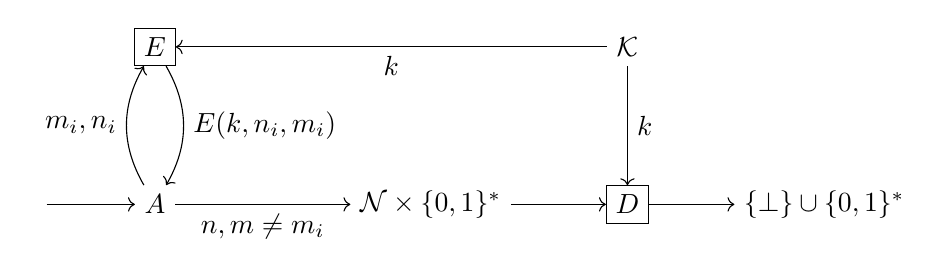
\begin{tikzpicture}
                \node (begin) at (-0.5, 0) {};
                \node (key) at (7, 2) {$\mathcal{K}$};
                \node (A) at (1, 0) {$A$};
                \node [shape = rectangle, draw = black] (X) at (1, 2) {$E$};
                \node (end) at (4.5, 0) {$\mathcal{N} \times \{ 0, 1 \}^*$};
                \node [shape = rectangle, draw = black] (verify) at (7, 0) {$D$};
                \node (result) at (9.5, 0) {$\{ \perp \} \cup \{ 0, 1 \}^*$};
    
                \draw [->] (begin) -- (A);
                \draw [->] (A) -- (end) node [midway, below] {$n, m \neq m_i$};
                \draw [->] (key) -- (X) node [midway, below] {$k$};
                \draw [->] (A) to [bend left] node [left, midway] {$m_i, n_i$} (X);
                \draw [->] (X) to [bend left] node [right, midway] {$E(k, n_i, m_i)$} (A);
                \draw [->] (end) -- (verify);
                \draw [->] (verify) -- (result);
                \draw [->] (key) -- (verify) node [midway, right] {$k$};
            \end{tikzpicture}
        \end{center}
    \end{definition}

    \vspace{10pt}

    \begin{itemize}
        \item Definitions emerge, change, and die more than people think
    \end{itemize}
\end{frame}

\begin{frame}
    \frametitle{Session Key distribution}

    \begin{center}
        We'll skip this
    \end{center}

\end{frame}

\begin{frame}
    \frametitle{Random oracle model}

    We assume the existence of a \emph{idealized hash function} (or random oracle) $H: \{ 0, 1 \}^* \to \{ 0, 1 \}^n$.
    \begin{center}
        \includegraphics<1>[height = 0.5\textheight]{ro0.pdf}
        \includegraphics<2>[height = 0.5\textheight]{ro1.pdf}
        \includegraphics<3>[height = 0.5\textheight]{ro2.pdf}
        \includegraphics<4>[height = 0.5\textheight]{ro3.pdf}
    \end{center}

    \begin{itemize}
        \item Defining and modelling are different, but similar
    \end{itemize}
\end{frame}

\begin{frame}
    \frametitle{References}
    \printbibliography
\end{frame}
\end{document}